\documentclass{beamer}

\usetheme{default}
\begin{document}

\title{Element-centered layout}

\subtitle{in WxFactory}
\begin{frame}
    \titlepage
\end{frame}

\begin{frame}{Intro}
\begin{itemize}
    \item Panel-centered layout (old)
    \item Element-centered layout (new)
    \item Performance comparison
    \item Boundary storage
    \item Next steps
\end{itemize}
\end{frame}

\begin{frame}{Panel-centered layout}
\begin{figure}
    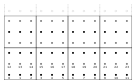
\includegraphics[scale=0.7]{img/variable_storage}
    \caption{Each row in the data array is made by concatenating the corresponding row of solution points of
             each element in a certain row of that tile (along axis $i$).
             Contiguous rows are for a single variable (e.g. pressure).}
\end{figure}
\end{frame}

\begin{frame}{Panel-centered layout}
\begin{columns}
\column{0.5\textwidth}
Good for
    \begin{itemize}
        \item Processing along the horizontal axis (e.g. extrapolation)
        \item Global grid operations
        \item Viewing data
    \end{itemize}

\column{0.5\textwidth}
Bad for
    \begin{itemize}
        \item Processing along the vertical axis (e.g. extrapolation)
        \item Element-wise operations in general
    \end{itemize}
\end{columns}
\end{frame}

\begin{frame}{Element-centered layout}
\begin{figure}
    \includegraphics[scale=0.7]{img/elem_wise_layout}
    \caption{Data points within an element are contiguous in memory.}
\end{figure}
\end{frame}

\begin{frame}{Performance comparison}
    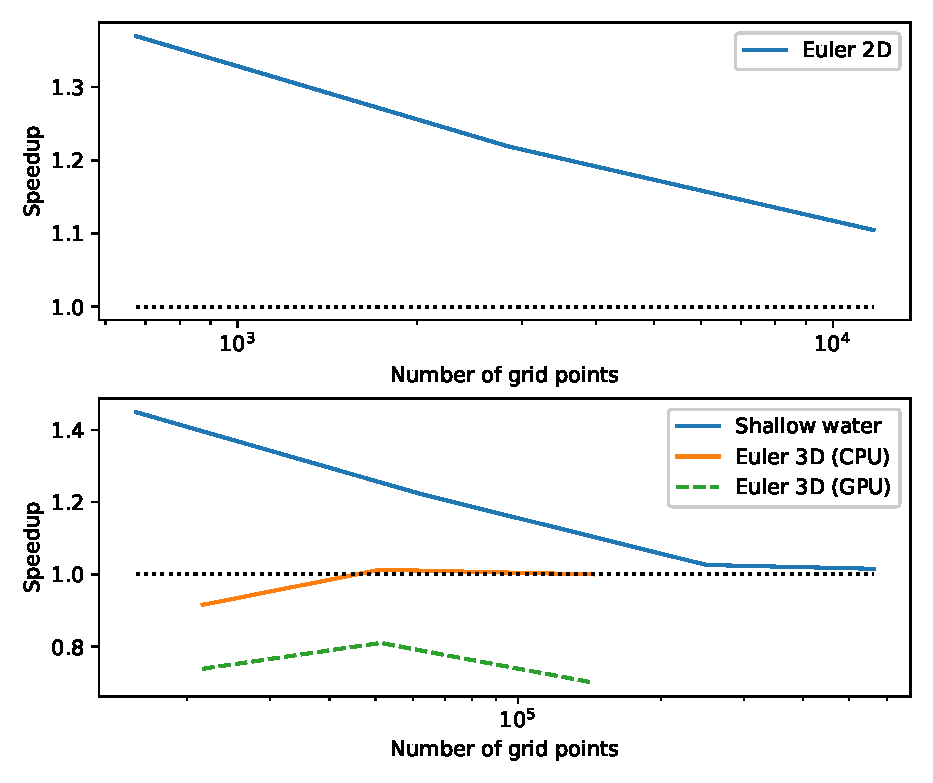
\includegraphics[scale=0.66]{img/layout_perf.eps}
\end{frame}

\begin{frame}{Discussion}{RHS operations}
\begin{itemize}
    \item Extrapolation
    \item Pointwise flux (layout independent)
    \item Flux divergence
    \item Riemann flux
    \item Forcing terms (layout independent)
\end{itemize}
\end{frame}

\begin{frame}{Extrapolation and flux divergence}
\begin{itemize}
    \item Old grid: fast in one direction, slow in the other(s)
    \item New grid: similar for each direction, should be overall faster if we compute all directions at once
        \begin{itemize} \item But we don't do that for extrapolation (yet). To be discussed \end{itemize}
    \item Independent of polynomial degree
\end{itemize}
\end{frame}

\begin{frame}{Riemann flux}
\begin{itemize}
    \item Should have similar performance in all directions
    \item New grid: probably depends on how we store boundaries
    \item With higher order, there are less boundaries, so less computation
\end{itemize}
\end{frame}

\begin{frame}{Boundary storage}
\begin{itemize}
    \item All in one array
    \begin{itemize}
        \item Good for extrapolation
        \item Bad for Riemann
    \end{itemize}
    \item All in separate arrays (4 in 2D, 6 in 3D)
        \begin{itemize} \item Opposite performance implications \end{itemize}
    \item 1 array per direction
        \begin{itemize} \item What we are currently doing \end{itemize}
    \item Layout considerations
    \begin{itemize}
        \item Impact on Riemann solve?
        \item What to do in 3D, where element boundaries are 2D
    \end{itemize}
\end{itemize}
\end{frame}

\begin{frame}{Next steps}
\begin{itemize}
    \item Write entire RHS in CUDA/C++ kernels
    \item Profile and optimize
    \item Explore boundary storage options
\end{itemize}
\end{frame}

\end{document}
